% vim:ts=4:sw=4
%
% Copyright (c) 2008-2009 solvethis
% Copyright (c) 2010-2015 Casper Ti. Vector
% Public domain.
%
% 使用前请先仔细阅读 pkuthss 和 biblatex-caspervector 的文档,
% 特别是其中的 FAQ 部分和用红色强调的部分。
% 两者可在终端/命令提示符中用
%   texdoc pkuthss
%   texdoc biblatex-caspervector
% 调出。

% 采用了自定义的(包括大小写不同于原文件的)字体文件名,
% 并改动 ctex.cfg 等配置文件的用户请自行加入 nofonts 选项;
% 其它用户不用加入 nofonts 选项,加入之后反而会产生错误。
\documentclass[UTF8]{pkuthss}

% 使用 biblatex 排版参考文献,并规定其格式(详见 biblatex-caspervector 的文档)。
% 这里按照英文文献在前,中文文献在后排序(“sorting = ecnty”);
% 若需按照中文文献在前,英文文献在后排序,请设置“sorting = centy”;
% 若需按照引用顺序排序,请设置“sorting = none”。
\usepackage[backend = biber, style = caspervector, utf8, sorting = none]{biblatex}

% 按学校要求设定参考文献列表中的条目之内及之间的距离。
\setlength{\bibitemsep}{3bp}
% 对于 linespread 值的计算过程有兴趣的同学可以参考 pkuthss.cls。
\renewcommand*{\bibfont}{\zihao{5}\linespread{1.27}\selectfont}

% 设定文档的基本信息。
\pkuthssinfo{
	cthesisname = {博士研究生学位论文}, ethesisname = {Doctor Thesis},
	ctitle = {测试文档}, etitle = {Test Document},
	cauthor = {某某},
	eauthor = {Test},
	studentid = {0123456789},
	date = {某年某月},
	school = {某某学院},
	cmajor = {某某专业}, emajor = {Some Major},
	direction = {某某方向},
	cmentor = {某某教授}, ementor = {Prof.\ Somebody},
	ckeywords = {其一,其二}, ekeywords = {First, Second}
}
% 载入参考文献数据库(注意不要省略“.bib”)。
\addbibresource{thesis.bib}

% 普通用户可删除此段。
\usepackage{color}
\def\pkuthssffaq{%
	\emph{\textcolor{red}{pkuthss 文档模版最常见问题:}}

	\texttt{\string\cite}、\texttt{\string\parencite} %
	和 \texttt{\string\supercite} 三个命令分别产生%
	未格式化的、带方括号的和上标且带方括号的引用标记:%
	\cite{test-en},\parencite{test-zh}、\supercite{test-en, test-zh}。

	若要避免章末空白页,请在调用 pkuthss 文档类时加入 \texttt{openany} 选项。

	如果编译时不出参考文献,
	请参考 \texttt{texdoc pkuthss}“问题及其解决”一章
	“其它可能存在的问题”一节中关于 biber 的说明。
}

\begin{document}
	% 以下为正文之前的部分,默认不进行章节编号。
	\frontmatter
	% 此后到下一 \pagestyle 命令之前不排版页眉或页脚。
	\pagestyle{empty}
	% 自动生成封面。
	\maketitle

	% 此后到下一 \pagestyle 命令之前正常排版页眉和页脚。
	% 封面要求单面打印,故需新开右页,此处已一并实现。
	\cleardoublepage
	\pagestyle{plain}
	% 重置页码计数器,用大写罗马数字排版此部分页码。
	\setcounter{page}{0}
	\pagenumbering{Roman}

	% 版权声明。
	\specialchap{版权声明}

任何收存和保管本论文各种版本的单位和个人,
未经本论文作者同意,不得将本论文转借他人,
亦不得随意复制、抄录、拍照或以任何方式传播。
否则一旦引起有碍作者著作权之问题,将可能承担法律责任。

% 若需排版二维码,请将二维码图片重命名为“barcode”,
% 转为合适的图片格式,并放在当前目录下,然后去掉下面 3 行的注释。
%\vfill\noindent
%\includegraphics[height = 5em]{barcode}


	% 中英文摘要。
	\begin{cabstract}
近年来,计算机技术的发展使得移动设备逐渐普及,通信技术的发展使得互联网无处不在。在这样的条件下,通过网络随时随地观看视频成为可能,而且逐渐发展为视频内容消费的主要形式。这种无需先下载好全部视频数据而是一边下载一边播放的技术称为视频流媒体。视频流媒体的相关应用,如按需点播、实时直播、在线教育、视频会议等,已经成为人们生活中不可或缺的部分。在这前所未有的机遇同时,视频流媒体也面临着网络异构性和带宽波动的挑战。为应对这一挑战,视频流媒体系统需要能够根据不同的网络条件自动调整所发送的数据码率,以适应带宽的变化。本文\footnote{本研究得到国家自然科学基金(项目编号61271020)和国家科技支撑计划(项目编号2014BAK10B02) 资助。}从数据源和数据传输过程两方面入手,结合点播和直播这两种应用模式,对自适应视频流媒体中的关键技术进行了全面深入的研究。首先,本文针对可伸缩视频数据源提出了新的失真模型和码流截取方案,在支持可变码率的同时提供尽可能高的视频质量;其次,本文为视频点播系统设计了新的码率自动调整策略,用控制论的方法来解决适应带宽变化的问题;最后,本文详细分析了现在非常流行的视频直播系统的传输过程,结合直播的特点提出了数据上传时的码率自适应算法。本文主要的创新性贡献可以归纳为如下三个部分:
\begin{enumerate}
\item {采用线性误差模型的可伸缩视频码流截取方案}\\
作为码率适应带宽波动的前提条件,视频流媒体中的数据源需要能够灵活调整。可伸缩视频编码将数据划分为基本层和增强层,通过丢弃增强层的数据包来实现即时码率变化。从完整的可伸缩码流中丢弃部分数据得到一个子流的过程称为码流截取。本文以最小化特定截取码率限制下的视频失真为目标,首先提出了一个线性误差模型来估计丢弃任意数据包组合带来的失真变化,然后利用它设计了一个贪心型算法来根据每个数据包的码率和失真影响对其赋优先级,作为截取过程中丢包的顺序。相比于参考软件,这一码流截取方案能够在同样的复杂度和码率限制下取得更高的视频质量。
\item {基于PID控制思想的点播系统码率自适应算法}\\
自适应视频流媒体中的另一个关键问题是传输过程中的码率调整策略,即在可用带宽不断变化的情况下,决定何时调整码率并确定调整到多少。本文基于经典的比例-积分-微分(PID)控制思想,提出了一个综合考虑带宽的历史状况、当前状态和未来趋势的码率自适应算法,既能充分利用带宽,传输较高的视频质量,又能减小带宽波动的影响,保证视频质量的平滑性。该算法集成在了苹果公司QuickTime流媒体服务器的开源版本上,并在实际应用中取得了很好的效果。
\item {基于数据缓冲区分析的直播系统码率自适应算法}\\
在视频直播中,由于数据是实时产生的,其传输过程与视频点播有所不同。视频数据需要先上传到服务器,然后由服务器分发到观看者进行播放。本文为这个过程中的上传阶段增加了码率自适应的特性:首先通过详细分析系统整个传输过程中各个缓冲区的关系,建立了一个多缓冲区模型;然后把上述点播系统中用到的PID方法与多缓冲区模型相结合,提出0了一个有效的码率自适应算法。相比于没有自适应的上传过程,带宽的利用率得到了提升,观看者播放视频的连续性也得到了改善。
\end{enumerate}
\end{cabstract}

\begin{eabstract}
In recent years, the development of computer technology has made the mobile devices popular, and the communication technology has made the Internet accessible everywhere. Under such circumstances, watching videos at any time and any place becomes possible, and even an increasingly important way for people to consume video content. This is called video streaming, where the video can play as the data are being downloaded, before the entire file has been transmitted. Applications of video streaming, e.g., video on demand (VoD), live broadcasting, online education, and remote video conference, have become an indispensable part of people's life. Along with those opportunities, video streaming also has the big challenge brought about by the variety of networks. To cope with this challenge, the video streaming system should be able to adjust the video’s bitrate or quality according to the network condition. In other words, the video streaming system needs to be adaptive. In this paper, we investigate and solve the key problems in adaptive video streaming. First, focusing on the adaptive video streaming system based on the Scalable Video Coding (SVC) extension of the H.264/AVC video coding standard, this paper proposes a novel bitstream extraction scheme to provide highest possible video quality while supporting bitrate adjustment at the same time. Second, this paper designs a new rate adaptation algorithm for the VoD system, adjusting the bitrate to fit the current bandwidth from the control perspective. And finally, this paper analizes the transmission process of live video streaming in detail and proposes a rate adaptation algorithm for its uploading stage. The innovative contributions of this paper can be summarized as follows.
\begin{enumerate}
\item {Bitstream extraction scheme utilizing a linear error model}\\
As the prerequisite for adaptation, the data source in video streaming should be adjustable. SVC enables the flexible adjustment of bitrate by separating the video data into basic layer and enhancement layers and discarding the enhancement layer data packets as needed. The process of discarding some data from the whole SVC bitstream to obtain a substream is known as bitstream extraction. Aiming to minimize the distortion under the constraint of certain bitrate, a simple and effective linear error model is proposed and verified, which can be used to accurately estimate the distortion caused by discarding any combination of data packets from an SVC bitstream. Then utilizing this model, a greedy-like algorithm is designed to assign priority for each data packet according to its Rate-Distortion (R-D) impact, thus enabling optimized bitstream extraction. Comparing with the reference software, this extraction scheme achieves higher video quality with the same computational complexity and bitrate constraint.
\item {Rate adaptation algorithm for VoD systems based on the idea of PID control}\\
When and how to adjust the bitrate according to the bandwidth change is another important issue in adaptive video streaming. This paper proposes a rate adaptation algorithm based on the classical Proportional-Integral-Derivative (PID) controller. By monitoring and predicting past, current and future bandwidth information, the PID-based quality control algorithm is able to reduce quality fluctuation while still preserving a high quality level. The algorithm is integrated into the open source version of Apple's QuickTime streaming server and performs well in the practical applications.
\item {Rate adaptation algorithm for live streaming systems based on analysis of data buffers}\\
In live video streaming systems, the data are generated in real time; therefore, the transmission process is also different from that of VoD systems. The video data should first be uploaded to a server, then distributed to watchers by the server. This paper proposes to add adaptation to the uploading stage. A multi-buffer model is built based on analysis of the several data buffers during the transmission, and it is combined with the PID method to provide rate adaptation effectively. Compared with non-adaptive uploading, the bandwidth utilization is improved and the playback continuity is also increased.
\end{enumerate}
\end{eabstract}
	% 自动生成目录。
	\tableofcontents

	% 以下为正文部分,默认要进行章节编号。
	\mainmatter
	% 序言。
	\chapter{绪论}

\section{研究背景和意义}

进入二十一世纪以来,人们表示和传递信息的媒介从文本、声音扩展到了图像、视频。如今视频已经成为人们生产和生活中不可缺少的部分。另一方面,在计算机技术和通信技术的推动下,人们对网络的依赖和要求也越来越高。
智能手机、平板电脑等移动设备的普及,Wi-Fi、4G等无线网络的覆盖,让人们能够随时随地访问互联网。这样的环境催生并促进了一项技术的蓬勃发展,这就是视频流媒体。

视频流媒体简单来说就是通过网络在线播放视频。所谓流媒体,是指音视频等多媒体数据通过网络以连续稳定的流的形式传输到客户端的一系列技术、协议和方法的总称。在视频流媒体中,视频数据从服务器连续不断地传输到客户端,客户端可以一边接收一边播放,无需等待整个文件发送完毕。与下载方式相比,这种采用流式传输的视频播放具有显著的优点\supercite{Li2002},包括:1)启动延迟大大缩短,用户可以在等待几秒或十几秒的缓冲后就立即开始观看;2)视频数据不在客户端长时间驻留,不仅节省了用户存储空间,也一定程度上避免了内容版权保护问题;3)支持数据的实时生成和获取,大大扩展了视频应用场景的范围。正是由于其优秀的特性,视频流媒体得到了广泛的应用,逐渐成为人们消费视频内容的主要形式\supercite{Chen2013}。

视频流媒体应用按照其对实时性要求的不同可以分为点播和直播两大类。在点播应用中,内容提供商将预先制作好的视频放在服务器上,并发布内容的描述信息和链接,用户选择自己感兴趣的内容请求播放相应的视频。典型的例子是在线视频网站,如国外的YouTube\footnote{https://www.youtube.com/}、Netflix\footnote{https://www.netflix.com/},国内的优酷\footnote{http://www.youku.com/}、乐视\footnote{http://www.le.com/}等。大多在线教育网站如Coursera\footnote{https://www.coursera.org/}、网易公开课\footnote{http://open.163.com/}等也属于视频点播类应用。在直播应用中,视频数据则是通过现场录制实时生成的,上传到流媒体服务器之后再即时分发给观看者,具有很强的时效性。这类应用包括现在互联网上正兴起的秀场、游戏、生活类直播软件,以及已经很成熟的远程监控、视频会议等等。直播应用往往也会把实时事件的内容存储起来,后续以点播的形式继续提供。

网络条件的改善,采集与播放设备的普及,使得视频流媒体应用进入了一个高速增长的时期。根据Cisco的一项预测\footnote{http://www.cisco.com/c/en/us/solutions/collateral/service-provider/ip-ngn-ip-next-generation-network/white\_paper\_c11-481360.html},从2014年到2019年,视频流量在所有互联网流量中的占比将从64\%上升至80\%。路透社的一篇报道\footnote{http://www.reuters.com/article/us-internet-consumers-cisco-systems-idUSKBN0EL15E20140610}指出,在美国这一比例在2018年即将达到83\%。可见,视频流媒体正迎来一个高峰期。

在前所未有的机遇同时,视频流媒体也面临着网络异构和带宽波动所带来的严峻挑战。从网络构成来看,目前既存在几百kb/s速度的拨号或3G上网,又有几十Mb/s速度的局域网或光纤接入,而且随着移动通信网与Internet的融合,无线与有线网络的混联,网络异构性更加明显。视频流媒体的终端用户可能处于不同的网络中(例如有线网,Wi-Fi,蜂窝移动网络等),甚至有可能在观看视频的过程中从一种网络切换到到另一种网络(典型的例子是手机用户在Wi-Fi和4G网络之间的切换)。即使是在同一网络环境中,视频传输可用的带宽也会因为网络拥堵情况的变化而不断波动。

在这样的实际条件下,如果视频流媒体系统以恒定的速率传输数据,将很难或者不可能会给用户带来最好的视频观看体验。举例来说,如果设置一个较低的码率,则对应的视频质量不高,达不到带宽充足用户的满意度;而如果设置较高的码率,则对低带宽的用户或者在带宽波动较大的情况下,可能会导致视频无法流畅播放。因此,为应对这一挑战,视频流媒体系统需要能够根据不同的网络条件自动调整所发送视频的码率,以适应带宽的变化。换句话说,视频流媒体需要具备自适应性。

考虑到视频流媒体的广泛应用,通过加入自适应性来进一步改善视频流媒体服务质量,具有重要的现实意义。自适应视频流媒体的研究既受到了工业界的普遍关注,也成为了学术界的一大热点。

\section{研究框架和问题}

自适应视频流媒体的研究属于视频流媒体研究领域的一个子集。视频流媒体是视频与流媒体的结合,因此这个领域的研究也涉及包括编码和传输在内的多个方面。如图\ref{fig:research-framework}所示,视频流媒体的研究可以从系统模块的角度分为以下几个部分:

\begin{itemize}
	\item 数据源端的研究,一方面是进行高效的压缩编码,以尽可能少的数据表示尽可能高的视频质量;另一方面是提供具备灵活性的码流,支持码率的变化甚至考虑容错,等等。
	\item 传输过程的研究,即如何又快又好地将视频数据送给用户,包括改善网络状况以提高传输的吞吐量和可靠性,合理公平地利用带宽资源,根据带宽情况自适应地调整传输速率等。
	\item 客户终端的研究,即优化用户设备收到视频码流之后的播放阶段,包括如何快速解码,进行一些画质增强等后处理过程从而更好地显示,等等。
\end{itemize}

\begin{figure}[h]
	\centering
	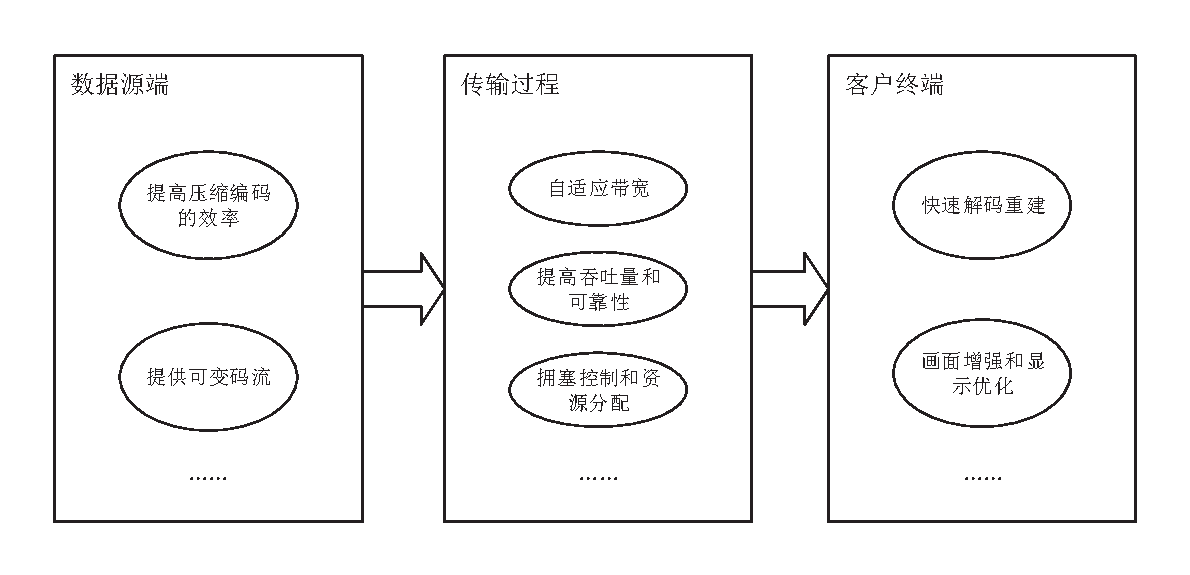
\includegraphics[width = 1.0\linewidth]{eps/research-framework}
	\caption{视频流媒体研究框架 \label{fig:research-framework}}
\end{figure}

在这一研究框架中,自适应视频流媒体主要涉及的是数据源端提供可变码率、传输过程中自动适应带宽这两个方面。虽然其他方面的研究工作,例如对编码效率的提升、对网络架构和协议的改进、在用户终端的解码优化等,也非常重要,但本文主要关注的是上述与自适性相关的两个方面(为构建高效自适应的实用视频流媒体系统所进行的客户端解码优化工作可参见本文作者已发表的其他论文)。

在视频流媒体系统中支持视频码率的可变性通常有两种选择。下面分别对其进行简单的介绍。

第一种选择是采取多码流的方法。多码流方法的原理很简单,就是预先编好不同码率的多个码流存放在服务器上,根据网络情况选取其中合适的一个进行传送。近年来兴起的HTTP动态自适应流媒体(Dynamic Adaptive Streaming over HTTP,  DASH)\supercite{Sodagar2011}就属于这类方法。如图\ref{fig:DASH}所示,DASH系统在服务器端提供不同码率的多个码流切片,客户端通过HTTP协议拉取数据,在某个时间段内可以选择性地接收这几个码流中任何一个的切片,通过在多码流之间切换来更改码率以适应带宽波动。

第二种选择是采用可伸缩视频编码\supercite{SVC-Overview}技术。作为国际视频编码标准H.264/AVC\supercite{H.264}的扩展之一,可伸缩视频编码的初衷就是在单个码流中加入伸缩性的支持,使其码率和视频质量能够根据需要改变。可伸缩视频码流中的数据被划分为基本层和增强层数据包,可以从中丢弃一部分增强层数据包而截取出一个子流,以牺牲视频质量的方式来降低码率。因此,用它来实现码率可变性正符合其设计目的。

\begin{figure}[t]
	\centering
	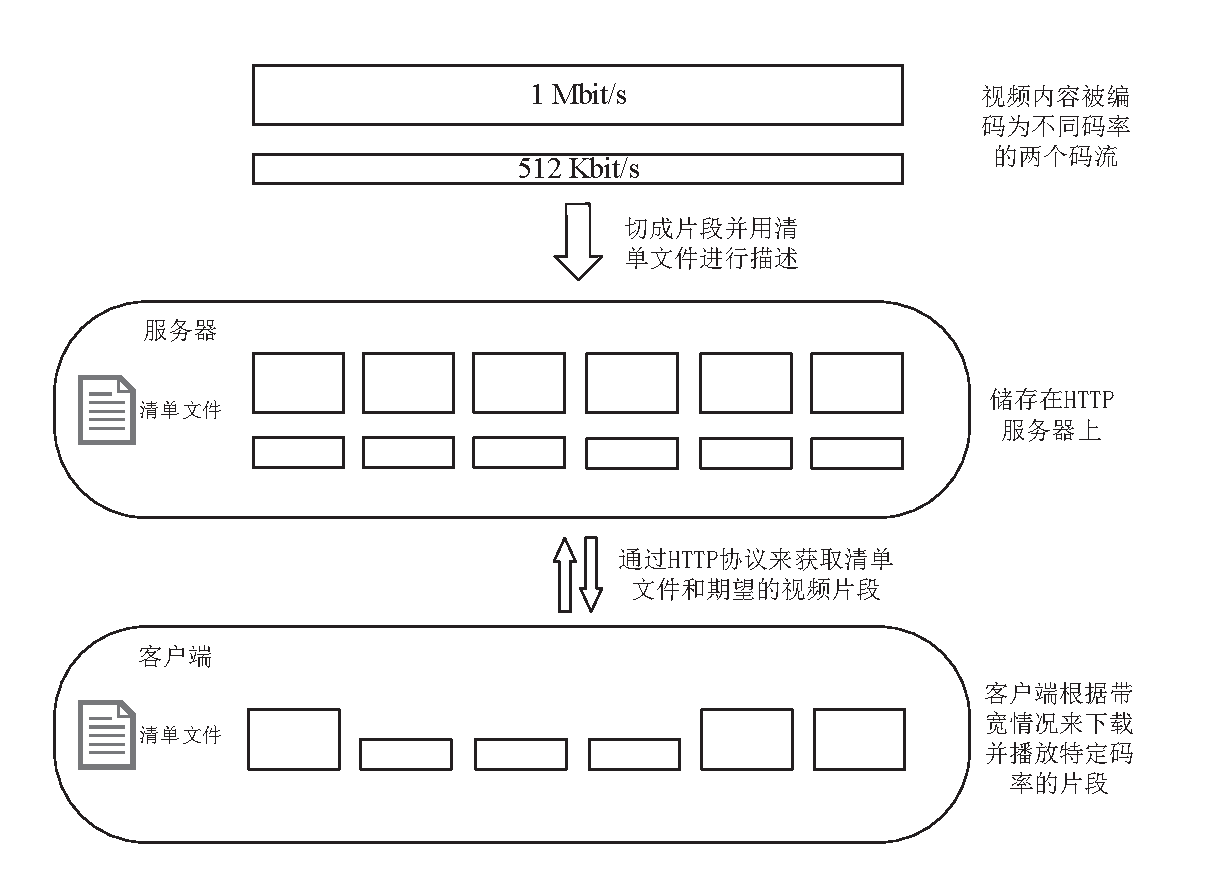
\includegraphics[width = 1.0\linewidth]{eps/DASH}
	\caption{DASH系统的工作原理示意图\label{fig:DASH}}
\end{figure}

多码流方案的优点是无需对已有的程序和系统做较大的改动,因此比较易于部署\supercite{Bouten2014}。很多商业视频网站(如YouTube、优酷等)已经用它实现了自适应功能。但是,多码流方案能提供的适应范围和粒度非常有限。例如,YouTube上的视频最多只提供144p、240p、360p、480p、720p和1080p这六个等级(参见图\ref{fig:13-1},其中右下角矩形框中显示了支持的等级),而优酷网上的视频大多只提供标清、高清、超清这三个画质(参见图\ref{fig:13}正中央的设置窗口)。此外,多个码流的编码和存储需要大量的计算资源和磁盘空间,使得时间和空间开销成倍增加。要想以合理的代价提供精细无缝的自适应性,就需要采用可伸缩视频编码的方案。可伸缩视频码流能够以非常小的数据粒度进行码率调整,而且性能分析表明可伸缩视频编码的压缩效率远高于同一内容多次编码的多码流方法\supercite{SVC-Performance}。正是因为这些优势,基于可伸缩视频编码来实现自适应视频流媒体从技术上来说是一个更好的方案,也吸引了学术界很多研究者的关注\supercite{Chuah2012, Zhu2013, Dan2013, Yang2014, Cicalo2014}。

\begin{figure}[!ht]
	\centering
	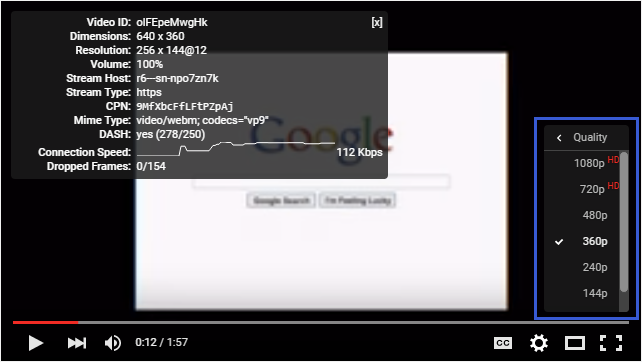
\includegraphics[width = 1.0\linewidth]{clip/13-1.png}
	\caption{YouTube视频码率自适应功能图示\label{fig:13-1}}
\end{figure}

\begin{figure}[!ht]
	\centering
	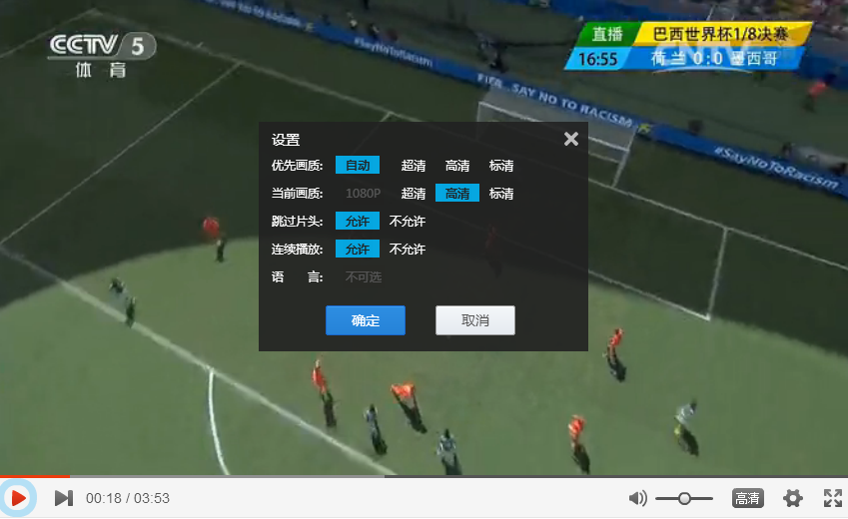
\includegraphics[width = 1.0\linewidth]{clip/13.png}
	\caption{优酷网视频码率自适应功能图示\label{fig:13}}
\end{figure}

本文的研究平台也主要是基于可伸缩视频编码的自适应流媒体系统。从图\ref{fig:research-framework}所示的研究框架中可以看出,采用可伸缩视频编码或是采用DASH之类的多码流方案,其区别只在于数据源端提供可变码率的方式不同。当可伸缩视频作为数据源时,在给定码率下选择丢弃哪些数据包,即如何最优地从整个码流中截取出一个子流用于发送是需要研究的问题之一。多码流作为数据源时则不存在这个问题。而对于在传输过程中如何自动调整码率以适应带宽的变化,却是二者共有的问题。这些问题的解决,是提高视频流媒体服务质量和用户体验的关键。

\section{本文研究内容和主要贡献}

本文结合视频流媒体所面临的挑战,对自适应视频流媒体中的关键技术进行研究,以更好地解决上面所提到的问题。首先,本文针对可伸缩视频数据源提出了新的失真模型和码流截取方案,在支持可变码率的同时提供尽可能高的视频质量;其次,本文为基于可伸缩视频编码的视频点播系统设计了新的码率自动调整策略,用控制论的方法来解决适应带宽变化的问题;最后,本文详细分析了现在非常流行的视频直播系统的传输过程,结合直播的特点提出了数据上传时的码率自适应算法。本文主要的创新性贡献可以归纳为如下三个部分:
\begin{enumerate}
\item {采用线性误差模型的可伸缩视频码流截取方案}\\
作为码率适应带宽波动的前提条件,视频流媒体中的数据源需要能够灵活调整。可伸缩视频编码技术通过将数据划分为基本层和增强层并丢弃增强层的数据包来实现即时码率变化。从完整的可伸缩码流中丢弃部分数据得到一个子流的过程称为码流截取。本文以最小化特定截取码率限制下的视频失真为目标,首先提出了一个线性误差模型来估计丢弃任意数据包组合带来的失真变化,然后利用它设计了一个贪心型算法来根据每个数据包的码率和失真影响对其赋优先级,作为截取过程中丢包的顺序。相比于参考软件,这一码流截取方案能够在同样的复杂度和码率限制下取得更高的视频质量。
\item {基于PID控制思想的点播系统码率自适应算法}\\
自适应视频流媒体中的另一个关键问题是传输过程中的码率调整策略,即在可用带宽不断变化的情况下,决定何时调整码率并确定调整到多少。本文基于经典的比例-积分-微分(Proportional-Integral-Derivative,PID)控制思想,提出了一个综合考虑带宽的历史状况、当前状态和未来趋势的码率自适应算法,既能充分利用带宽,传输较高的视频质量,又能减小带宽波动的影响,保证视频质量的平滑性。该算法集成在了苹果公司QuickTime流媒体服务器的开源版本上,并在实际应用中取得了很好的效果。
\item {基于缓冲区分析的直播系统码率自适应算法}\\
在视频直播中,由于数据是实时产生的,其传输过程与视频点播有所不同。视频数据需要先上传到服务器,然后由服务器分发到观看者进行播放。本文为这个过程中的上传阶段增加了码率自适应的特性:首先通过详细分析系统整个传输过程中各个缓冲区的关系,建立了一个多缓冲区模型;然后把上述点播系统中用到的PID方法与多缓冲区模型相结合,提出了一个有效的码率自适应算法。相比于没有自适应的上传过程,带宽的利用率得到了提升,视频播放的连续性也得到了改善。
\end{enumerate}

\section{本文的结构安排}

本文共分为六章,后续章节具体内容安排如下。

第二章概述视频流媒体领域的研究基础和相关工作。首先对视频编码和流式传输的基础知识进行简要介绍,为后文内容做准备;然后对本文所要研究的可伸缩视频码流截取、传输中的码率自适应这两个问题进行具体描述,并分析已有的相关工作。

第三章讨论采用线性误差模型的码流截取方案。首先针对可伸缩视频推导并验证线性误差模型,然后介绍采用该模型的失真估计方法和以码率失真影响为度量标准的优先级赋值算法。最后展现并分析所提出的码流截取方案的实验结果。

第四章讨论基于PID控制思想的点播系统码率自适应算法。首先对PID控制器做简单的介绍,然后将PID模型运用到视频传输中的码率调整策略,提出了一个新颖的码率自适应算法。该算法被集成在了苹果公司QuickTime流媒体服务器的开源版本中,其有效性通过对比实验得到了验证。

第五章讨论针对直播系统的码率自适应算法。首先详细分析了直播系统的传输过程,提出了一个多缓冲区模型;然后将其与PID方法相结合,选取合适的系统变量实现了上传过程的码率自适应算法,改善了带宽利用率和观看者的播放连续性。

第六章总结全文内容并对未来工作和应用前景进行展望。
	% 各章节。
	% vim:ts=4:sw=4
% Copyright (c) 2014 Casper Ti. Vector
% Public domain.

\chapter{章节}
% 中文测试文字。
\pkuthssffaq


	% 结论。
	\chapter{总结和展望}
本章总结全文并展望未来工作。

	% 正文中的附录部分。
	\appendix
	% 排版参考文献列表。
	\printbibliography[
		% 使“参考文献”出现在目录中;如果同时要使参考文献列表参与章节编号,
		% 可将“bibintoc”改为“bibnumbered”。
		heading = bibintoc,
		% 单独设定排序方案。此设定会局部覆盖之前的全局设置。
		% 注:只有同时使用 2.x 或之后版本的 biblatex 和相应兼容版本的 biber,
		% 才能对每个 \printbibliography 命令采用不同的排序方案,
		% 否则只能在载入 biblatex 宏包时就(全局)指定排序方案。
		% 在这样的情况下,请去掉所有的 sorting 选项,否则可能出错。
		% 此外,biblatex 3.0 中 \printbibliography 的 sorting 选项失效,
		% 详见 biblatex-caspervector 的文档。
		sorting = ecnty
	]
	% 各附录。
	% vim:ts=4:sw=4
% Copyright (c) 2014 Casper Ti. Vector
% Public domain.

\chapter{附件}
% 中文测试文字。
\pkuthssffaq



	% 以下为正文之后的部分,默认不进行章节编号。
	\backmatter
	% 致谢。
	\chapter{致谢}

感谢计算机所的老师、同学等所有在我读博士期间关心帮助过我的人。


	% 原创性声明和使用授权说明。
	{
	\CTEXsetup[
		format+ = {\centering}, beforeskip = {40bp}, afterskip = {15bp}
	]{section}

	\specialchap{北京大学学位论文原创性声明和使用授权说明}
	\mbox{}\vspace*{-3em}
	\section*{原创性声明}

	本人郑重声明:
	所呈交的学位论文,是本人在导师的指导下,独立进行研究工作所取得的成果。
	除文中已经注明引用的内容外,
	本论文不含任何其他个人或集体已经发表或撰写过的作品或成果。
	对本文的研究做出重要贡献的个人和集体,均已在文中以明确方式标明。
	本声明的法律结果由本人承担。
	\vskip 1em
	\rightline{%
		论文作者签名:\hspace{5em}%
		日期:\hspace{2em}年\hspace{2em}月\hspace{2em}日%
	}

	\section*{学位论文使用授权说明}

	本人完全了解北京大学关于收集、保存、使用学位论文的规定,即:
	\begin{itemize}
		\item 按照学校要求提交学位论文的印刷本和电子版本;
		\item 学校有权保存学位论文的印刷本和电子版,
			并提供目录检索与阅览服务,在校园网上提供服务;
		\item 学校可以采用影印、缩印、数字化或其它复制手段保存论文;
		\item 因某种特殊原因需要延迟发布学位论文电子版,
			授权学校在 $\Box$\nobreakspace{}一年 /
			$\Box$\nobreakspace{}两年 /
			$\Box$\nobreakspace{}三年以后在校园网上全文发布。
	\end{itemize}
	\centerline{(保密论文在解密后遵守此规定)}
	\vskip 1em
	\rightline{%
		论文作者签名:\hspace{5em}导师签名:\hspace{5em}%
		日期:\hspace{2em}年\hspace{2em}月\hspace{2em}日%
	}

	% 若需排版二维码,请将二维码图片重命名为“barcode”,
	% 转为合适的图片格式,并放在当前目录下,然后去掉下面 2 行的注释。
	%\vfill\noindent
	%\includegraphics[height = 5em]{barcode}
}


\end{document}

